\documentclass[a4paper, 10pt]{article}
\linespread{1.33}
% ┌─────────────────────┐
% │     preamble.tex    │
% └─────────────────────┘

% ══════════ [1] Basic document settings ══════════
\usepackage{fullpage}
\usepackage{geometry}
\geometry{
    top = 2cm,
    bottom = 4.5cm,
    left = 2.5cm,
    right = 2.5cm
}
\usepackage{lastpage}

\usepackage{xcolor}
\usepackage{graphicx}
\usepackage{tikz}
\usepackage{pgfplots}

\usepackage{enumerate}
\usepackage{sectsty}
\subsectionfont{\color{blue}}
\usepackage{enumitem}
\usepackage{array}
\newcolumntype{P}[1]{>{\centering\arraybackslash}p{#1}}

\usepackage{fourier-orns}
\usetikzlibrary{decorations.text}
\pgfplotsset{compat = newest}
\newcommand{\seprule}{
    \vspace*{1.5em}
    \vspace{-8pt}\hrulefill
    \raisebox{-2.1pt}{\quad\decofourleft\decotwo\decofourright\quad}\hrulefill
    \vspace*{1.5em}
}

\usepackage{hyperref}
\hypersetup{
  colorlinks=true,
  linkcolor=blue,
  linkbordercolor={0 0 1},
  urlcolor=blue
}

\usepackage{fancyhdr}
\usepackage[]{mdframed}

\renewcommand{\thesubsection}{\S{} \arabic{section}.\arabic{subsection}}

% ══════════ [2] Math packages ══════════
\usepackage{amsmath}
\usepackage{amsthm}
\usepackage{amsfonts}
\usepackage{amssymb}
\usepackage{amscd}
\usepackage{mathrsfs}
\usepackage{cancel}

% ══════════ [3] Miscellaneous & Fonts ══════════
\setlength{\parindent}{0.0in}
\setlength{\parskip}{0.05in}
\renewcommand{\footrulewidth}{0.4pt}

\usepackage{mathpazo}
\usepackage{domitian}
\usepackage[T1]{fontenc}
\let\oldstylenums\oldstyle
\setmonofont[Scale = 0.8]{DejaVu Sans Mono}

% ══════════ [4] amsthm setup ══════════

\newtheorem{theorem}{Theorem}[section]
\newtheorem{corollary}[theorem]{Corollary}
\newtheorem{lemma}[theorem]{Lemma}

\theoremstyle{definition}
\newtheorem{definition}[theorem]{Definition}

\theoremstyle{remark}
\newtheorem*{remark}{Remark}

\theoremstyle{definition}
\newtheorem{obs}[theorem]{Observation}

\theoremstyle{definition}
\newtheorem{exercise}[theorem]{Exercise}
\newmdtheoremenv[innertopmargin = 8pt,
                 innerbottommargin = 10pt]{exer}[theorem]{Exercise}

\theoremstyle{definition}
\newtheorem{example}[theorem]{Example}
% ┌─────────────────────┐
% │   usercommand.tex   │
% └─────────────────────┘

% ══════════ [1] short-hand notations ══════════
\newcommand{\mbf}{\mathbf}
\newcommand{\mrm}{\mathrm}
\newcommand{\mca}{\mathcal}
\newcommand{\msc}{\mathsc}
\newcommand{\mbb}{\mathbb}
\newcommand{\msf}{\mathsf}

\newcommand{\tbf}{\textbf}
\newcommand{\tit}{\textit}

\newcommand{\eps}{\epsilon}
\newcommand{\kB}{k_{\mathrm{B}}}
\def\dbar{{\mathchar'26\mkern-12mu d}}
\newcommand{\contradiction}{\ensuremath{{\Rightarrow\mspace{-2mu}\Leftarrow}}}
\newcommand{\im}{\mathrm{im}\,}
\renewcommand{\d}{\mathrm{d}}

\renewcommand\qedsymbol{$\blacksquare$}

\newcommand\lecturenumber{03}
\newcommand\lecturedate{Oct 25, 2024}

\pagestyle{fancyplain}
\headheight 40pt
\lhead{Lecture \lecturenumber\\CNBC Deep Learning Subgroup}
\rhead{Riemannian Geometry for Deep Learning \\\lecturedate}
\cfoot{Fall 2024, SNU}
\rfoot{\small\thepage}
\headsep 1.5em

\begin{document}
\setcounter{section}{2}
\setcounter{subsection}{0}
\setcounter{theorem}{0}

\section{Manifolds: Heuristic Introduction}

\begin{remark}
    Both Euclidean space($\mbb{R}^{3}$ with metric $\delta_{\mu\nu}$) and Minkowski space($\mbb{R}^{4}$ with metric $\eta_{\mu\nu}$) are \tit{flat}. In other words, those spaces have \tbf{constant metric}, regardless of the point you are interested in.
\end{remark}

\begin{definition}[Polar coordinates in 2D]
    The \tbf{polar coordinates} in $\mbb{R}^{2}$ is represented by $(r,\phi)$ with $0\leq r < \infty$ and $0 \leq \phi \leq 2\pi$. Then
    \[ x = r\cos\phi, \quad y = r\sin\phi \]
    and
    \[ r = \sqrt{x^{2} + y^{2}}, \quad \phi = \arctan\frac{y}{x} \]
    Note that the coordinate system is well-defined except at $r = 0$. Let's compute the metric.
    \begin{align*}
        \d s^{2} = \d x^{2} + \d y^{2} &= (\d r\cos\phi - r\sin\phi\d \phi)^{2} + (\d r\sin\phi + r\cos\phi\d{\phi})^{2} \\
        &= \d{r}^{2} + r^{2}\d\phi^{2} = \begin{bmatrix}\d{r} & \d\phi\end{bmatrix}\begin{bmatrix}1 & 0 \\ 0 & r^{2}\end{bmatrix}\begin{bmatrix}\d{r} \\ \d\phi\end{bmatrix}
    \end{align*}
    Hence,
    \[ g_{\mu\nu} = \begin{bmatrix}1 & 0 \\ 0 & r^{2}\end{bmatrix} \quad\text{or}\quad g_{rr} = 1,\; g_{r\phi} = g_{\phi r} = 0,\; g_{\phi\phi} = r^{2} \]
    The metric changes upon the location of point $p \in \mbb{R}^{3}$.
\end{definition}
\begin{definition}[Spherical polar coordinates]
    The \tbf{spherical polar coordinates} in $\mbb{R}^{3}$ is represented by $(r,\theta,\phi)$ with $0\leq r <\infty$, $0\leq\theta\leq\pi$ and $0\leq\phi\leq 2\pi$. Then
    \[ x = r\sin\theta\cos\phi,\; y = r\sin\theta\sin\phi,\; z = r\cos\theta \]
    and
    \[ r = \sqrt{x^{2} + y^{2} + z^{2}},\; \theta = \arctan\frac{\sqrt{x^{2}+y^{2}}}{z},\; \phi = \arctan\frac{y}{x} \]
    The interval becomes
    \begin{align*}
        \d{s}^{2} &= \d{x}^{2} + \d{y}^{2} + \d{z}^{2} = \d{r}^{2} + r^{2}\d{\theta}^{2} + r^{2}\sin^{2}\theta\d{\phi}^{2} \\
        &= \begin{bmatrix} \d{r} & \d{\theta} & \d{\phi} \end{bmatrix}\begin{bmatrix} 1 & 0 & 0 \\ 0 & r^{2} & 0 \\ 0 & 0 & r^{2}\sin^{2}\theta \end{bmatrix}\begin{bmatrix} \d{r} \\ \d{\theta} \\ \d{\phi} \end{bmatrix}
    \end{align*}
    Hence,
    \[ g_{\mu\nu} = \begin{bmatrix} 1 & 0 & 0 \\ 0 & r^{2} & 0 \\ 0 & 0 & r^{2}\sin^{2}\theta \end{bmatrix} \quad\text{or}\quad g_{rr} = 1,\; g_{\theta\theta} = r^{2},\; g_{\phi\phi} = r^{2}\sin^{2}\theta \]
    where all off-diagonal terms are zero.
\end{definition}
\newpage

% ===== ===== ===== ===== ===== ===== ===== ===== ===== ===== ===== =====

\begin{obs}
    Consider $\mbb{R}^{n}$ with coordinate system $x^{\mu}$ and metric $g$ ($\d{s}^{2} = g_{\mu\nu}\d{x}^{\mu}\d{x}^{\nu}$). Suppose that we define new \tit{local} coordinate system $\tilde{x}^{\mu}$ on a subspace of $\mbb{R}^{n}$.
    \[ \tilde{x}^{\mu} = h^{\mu}(x^{1},\cdots,x^{n}) \]
    We call this new coodinate system \tit{nice} if $\{h^{\mu}\}$ are invertible (in other words, $\{\tilde{h}^{\mu}\}$ exists such that $x^{\mu} = \tilde{h}^{\mu}(\tilde{x}^{1},\cdots,\tilde{x}^{n})$). We assume that $\{h^{\mu}\}$ and $\{\tilde{h}^{\mu}\}$ are sufficiently differentiable. The \tbf{transformation matrix} (or \tbf{Jacobian}) between those coordinates is
    \[ \frac{\partial\tilde{x}^{\mu}}{\partial{x}^{\nu}} = \frac{\partial{h}^{\mu}}{\partial{x}^{\nu}} := \Lambda^{\mu}{}_{\nu} \]
    Here, the metric $g$ and coordinate transformation $\Lambda$ are position-dependent. Those two are related via
    \begin{align*}
        \d{s}^{2} = g_{\mu\nu}\d{x}^{\mu}\d{x}^{\nu} &= g_{\mu\nu}\frac{\partial{x}^{\mu}}{\partial\tilde{x}^{\lambda}}\frac{\partial{x}^{\nu}}{\partial\tilde{x}^{\sigma}}\d\tilde{x}^{\lambda}\d\tilde{x}^{\sigma} \\
        &= \underbrace{(\Lambda^{-1})^{\mu}{}_{\lambda}g_{\mu\nu}(\Lambda^{-1})^{\nu}{}_{\sigma}}_{:= \tilde{g}_{\lambda\sigma}} \d\tilde{x}^{\lambda}\d\tilde{s}^{\sigma}
    \end{align*}
    In matrix notation, $(\Lambda^{-1})^{\msf{T}}g\Lambda^{-1} = \tilde{g}$.
\end{obs}
\begin{remark}
    Multiple local coordinate system can exist in one space!
\end{remark}

\seprule

\begin{example}[Unit sphere]
    Consider a unit sphere in $\mbb{R}^{3}$, $S^{2}$.
    \begin{enumerate}
        \item $S^{2}$ can be parametrized with spherical polar coordinates. However, we cannot represent entire $S^{2}$ with this coordinate system.
        \begin{itemize}
            \item[-] At $\phi = 0$ (or $\phi = 2\pi$), \tit{discontinuity} arises.
            \item[-] If we choose $\phi$ to increase more as we cross the $\phi = 2\pi$ line, \tit{uniqueness} problem arises (how do we know a point has $\phi$ or $\phi + 2\pi,\, \phi + 4\pi, \cdots$?).
            \item[-] At poles, $\phi$ values are ill-defined.
        \end{itemize}
        \item \tbf{Stereographic projection} maps a point on $S^{2}$, $P(x,y,z)$ to the point on $xy$-plane, $Q(X,Y,0)$ by drawing a straight line connecting a pole and $P$. The point where that line meets with $xy$-plane becomes $Q$. Such $Q$ is related to Cartesian (and spherical polar) coordinates by
        \[ X = \frac{x}{1-z} = \cot\frac{\theta}{2}\cos\phi,\; Y = \frac{y}{1-z} = \cot\frac{\theta}{2}\sin\phi \]
        \begin{itemize}
            \item[-] If we use North Pole as a reference, North Pole itself cannot be projected.
            \item[-] If we choose two points lying close to the pole, their stereographic projections will be located on widely different points.
        \end{itemize}
    \end{enumerate}
\end{example}
\newpage

% ===== ===== ===== ===== ===== ===== ===== ===== ===== ===== ===== =====

\begin{figure}[htbp!]
    \centering
    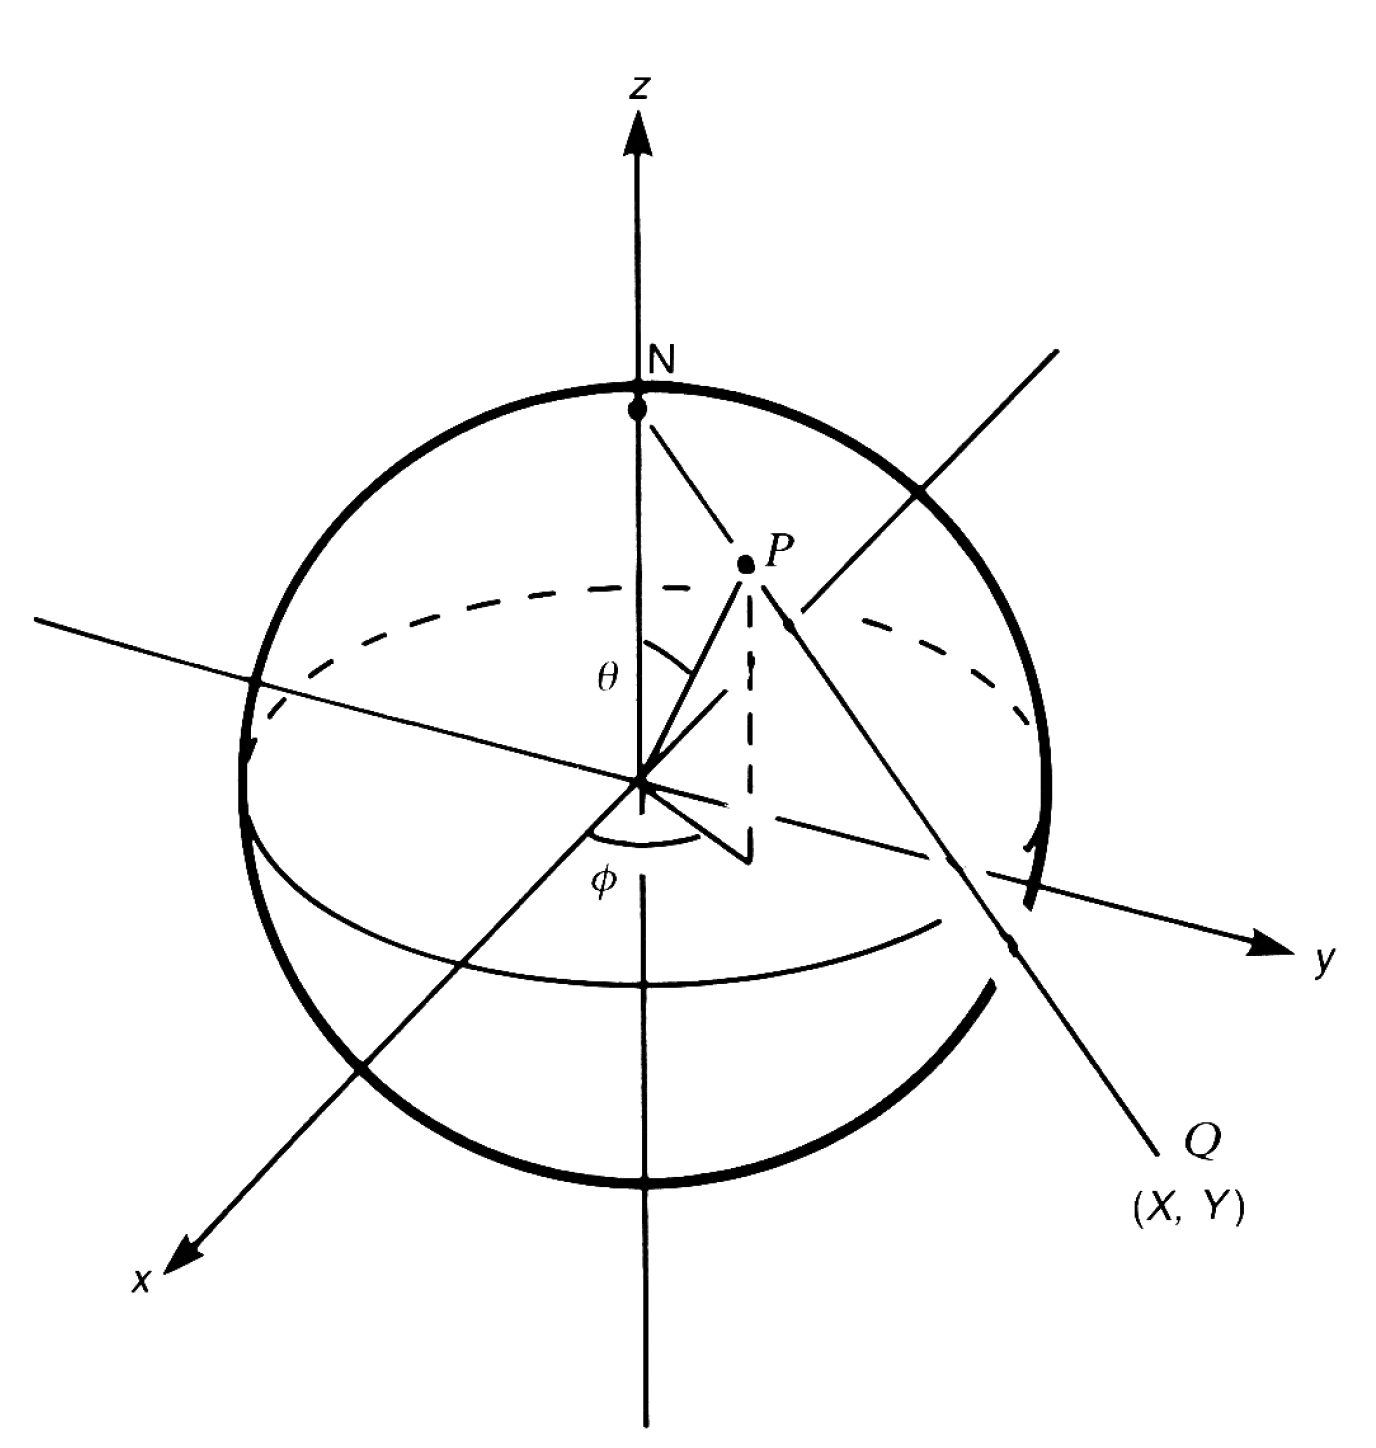
\includegraphics[width=0.5\linewidth]{../images/lecture03/3_01.png}
\end{figure}

\begin{obs}
    We cannot label the points on the sphere with a single coordinate system such that
    \begin{itemize}
        \item[(i)] Nearby points are mapped to nearby coordinates.
        \item[(ii)] Every point has unique coordinates.
    \end{itemize}
    Instead, define coordinates that satisfy requirements on a part of $S^{2}$ (by introducing two or more overlapping coordinate systems).
    \begin{itemize}
        \item[(i)] Nearby points are mapped to nearby coordinates(\tit{in at least one coordinate system}).
        \item[(ii)] Every point has unique coordinates(\tit{in each system that contains that point}).
        \item[(iii)] If two coordinate systems overlap, they are related to each other in a sufficiently \tit{smooth} way.
    \end{itemize}
\end{obs}

\end{document}
